\chapter{Environment Representation}\label{ch:environment.representation}

In this work, it is assumed that the drone has access to a simple representation of its environment. Therefore, the next step, before the implementation of navigation algorithms, is the creation of such a representation that can be exploited by the drone.

This chapter presents the simple representation designed for the environments, its characteristics, its use and the information that can be derived from it.

\section{Usefulness of a representation}

Any navigation system requires, in one way or another, knowledge of its environment. This knowledge can be built up entirely on the fly (\eg{} using SLAM with the appropriate sensors \cite{aguilar2017visual, bryson2007building}) or based on a priori knowledge (\eg{} using a predefined map of the environment).

In this project, the second option is chosen: a priori knowledge of the environment, in the form of a map, is available. Although this assumption may seem simplistic, it is in fact quite realistic for two reasons.

\begin{enumerate}
    \item As this work is part of several works on drones, the problem of mapping an environment is already addressed separately from this work. It is therefore plausible to assume that the results of that other work would be available for the navigation algorithms of this work.
    \item Without a priori knowledge of its environment, the drone can hardly learn to move from any starting point to any objective since it can not plan a path in advance. For example, when the drone comes to a turn, it will have no idea whether to turn left or right. It is possible to hardcode this information (via proper training of a Deep Learning model, for example), but the drone will only be limited to one possible path.
\end{enumerate}

A knowledge of the environment therefore allows the drone to navigate in the environment without being restricted to certain pre-defined fixed paths : it can predict a path from any starting point to any objective. The drone can also extract information from this path in advance: the number of turns and crossroads, their directions, the number of staircases to be crossed, the approximate distances to be covered, the potential other difficulties present (\eg{} a door to be crossed), but also keep an approximate trace of its position in the environment.

\section{Representation}

The environment must be represented in a way that can be used by the drone and the navigation algorithms. In order to optimize the computing time, the representation must be as light as possible and contain only the essential information useful for autonomous navigation (\ie{} the global structure of the environment, not every details it contains).

A known means in the field of robots to represent an environment is an \emph{occupancy grid}.

\subsection{Occupancy grid}\label{sec:05.occupancy.grid}

An occupancy grid \cite{wikipedia2021occupancygridmapping} is a grid, which can be represented via a matrix, discretizing the environment and where each location is marked with a value, belonging to the interval $[0, 1]$, indicating the probability of presence of an obstacle.

Within the framework of this work, a particular case of occupancy grid will be used: a \emph{binary occupancy grid}. In this case, the matrix representing the grid contains only two values: $0$ to indicate a free position and $1$ to indicate an occupied position (\eg{} a wall).

This representation implies a discretization of the environment. The smaller the step size chosen, the more accurate the representation will be, but it will be memory intensive and therefore slow to manipulate. As mentioned in Chapter \ref{ch:controllers}, the drone considered is not capable of extremely precise movement; it is therefore not necessary to have a representation accurate to the centimeter. As a good compromise between accuracy and simplicity, a $\SI{1}{\meter}$ step precision was chosen.

\begin{note}
    With an occupancy grid and a step precision of $\SI{1}{\meter}$, it may be difficult to represent precisely complex shapes (a circle, for example). In this project, only simple indoor environments (with simple shapes) are considered, so this is not really a problem.
\end{note}

\subsubsection{Two-dimensional representation}

The binary occupancy grid is a two-dimensional representation of the environment. Although the drone moves in 3 dimensions, this representation, in the context of this work, is sufficient.

Indeed, the environment considered (the corridors of the Montefiore Institute) is relatively simple. The drone will only very rarely have to modify its altitude (only for staircases, see Section \ref{sec:05.staircases.floors.management} for their management), and never in the context of path planning. It is not necessary to store the height of the environment in its representation; this would only make it more cumbersome and increase the processing time of the algorithms for nothing really useful.

\subsection{Implementation}

The implementation of the binary occupancy grid has been done in such a way that it can be easily created manually and easily exported and modified. In practice, the representation is stored in a text file (\texttt{.txt}) and is built based on several symbols explained in Table \ref{tab:05.environment.representation.symbols}.

\begin{table}[H]
    \centering
    \begin{tabular}{|c|p{10cm}|}
        \hline
        \textbf{Symbol} & \textbf{Function} \\ \hline
        \hline
        \texttt{.} & a free position \\ \hline
        \texttt{\#} & an occupied position \\ \hline
        \texttt{N, S, W, E} & the starting position of the drone, additionally representing its orientation (North, South, West, East) \\ \hline
        \texttt{B} & a battery station \\ \hline
        \texttt{*} & the objective to reach \\ \hline
        \texttt{+} & staircases that go up \\ \hline
        \texttt{-} & staircases that go down \\ \hline
    \end{tabular}
    \caption{Symbols used to represent characteristics of the representation of an environment.}
    \label{tab:05.environment.representation.symbols}
\end{table}

An example of a very simple environment representation is given in Figure \ref{fig:05.simple.environment.representation.txt}.

\begin{figure}[H]
    \centering
    \begin{minipage}[t]{0.135\textwidth}
        \begin{lstlisting}[style=defaultFrameTBNumber, gobble=12]
            ##########
            #E.....#*#
            #......#.#
            #......#.#
            #..#####.#
            #..#.....#
            #..#.....#
            #........#
            ##########
        \end{lstlisting}
    \end{minipage}
    \caption{Representation of a very simple environment in \texttt{.txt} format.}
    \label{fig:05.simple.environment.representation.txt}
\end{figure}

The representation in Figure \ref{fig:05.simple.environment.representation.txt}, when interpreted, results in a visual map shown in Figure \ref{fig:05.simple.environment.visual}.

\begin{figure}[H]
    \centering
    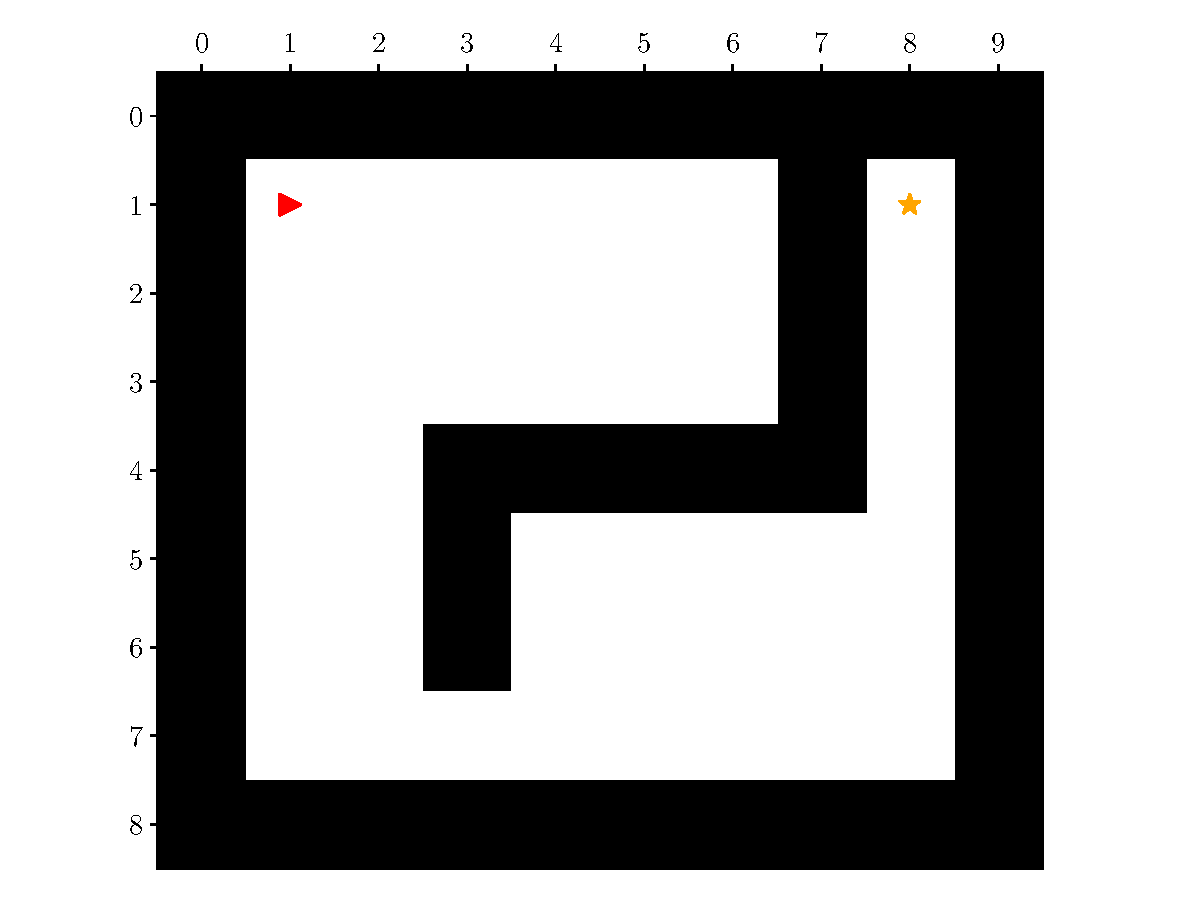
\includegraphics[width=0.5\textwidth]{resources/pdf/05/simple-environment/map.pdf}
    \caption{Visual representation of the simple environment described in Figure \ref{fig:05.simple.environment.representation.txt} where the red arrow represents the position and orientation of the drone and the yellow star represents its objective. Each free and occupied positions are shown, respectively, in white and black.}
    \label{fig:05.simple.environment.visual}
\end{figure}

The other symbols not used in this example (battery station, staircases) are used to add more complex features which will be explained in Section \ref{sec:05.features}.

\begin{note}
    Since the binary occupancy grid is represented by a matrix, it is mandatory that the environment is represented by a grid of $N \times M$ symbols. If the environment we want to represent is not rectangular in shape, the empty areas can be filled with non-free position symbols.
\end{note}

\section{Features}\label{sec:05.features}

The representation of the environment has several features that help the drone to navigate autonomously.

\subsection{Path planning}

Shortest path planning is one of the most important features. With a representation of its environment, the drone is able to move from any start point to any objective, provided that it can plan a path between these two points.

Very popular for its simplicity and efficiency, the \emph{A*} path planning algorithm \cite{hart1968formal, medium2017astar} was chosen. This algorithm allows the planning of a shortest path between a start node and an end node in a graph. For each node, the algorithm computes a cost defined as
\begin{equation}
    f = g + h
\end{equation}
where $g$ is the distance between the considered node and the start node and $h$ is an estimation of the distance, via a heuristic, between the considered node and the end node. The different nodes are then, during the iterations, considered or not by the algorithm according to their costs, the goal being to minimize the total cost of the path.

Considering that each location of the binary occupancy grid is a node of an undirected graph and that each node has 4 neighbors (top, bottom, left and right), the distance between a node and one of its neighbors (used to compute $g$) is set to $1$ and the heuristic $h$ chosen is the \emph{Euclidean norm} between two nodes, \ie{} for two nodes $n_1$ and $n_2$,
\begin{equation}
    h(n_1, n_2) = \sqrt{(n_{2_x} - n_{1_x})^2 + (n_{2_y} - n_{1_y})^2}
\end{equation}
where $\circ_x$ and $\circ_y$ are, respectively, the line and column of a node $\circ$ in the matrix.

The algorithm was tested on the simple environment \ref{fig:05.simple.environment.representation.txt} but also on a complex one. The obtained paths are presented in Figure \ref{fig:05.path.planning.examples}.

\begin{figure}[H]
    \centering
    \begin{subfigure}[b]{0.50\textwidth}
        \centering
        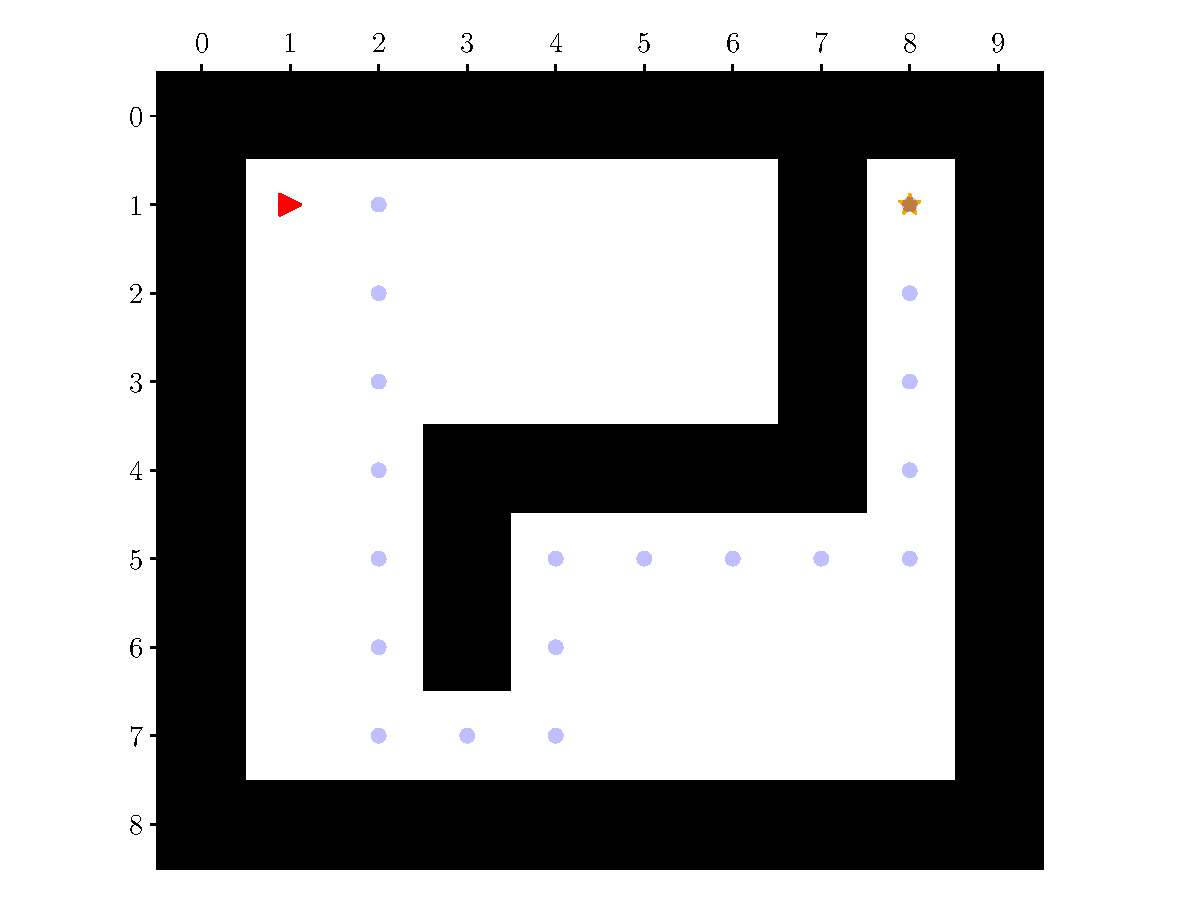
\includegraphics[width=\textwidth]{resources/pdf/05/simple-environment/path.pdf}
        \caption{Simple environment}
        \label{fig:05.path.planning.examples.simple}
    \end{subfigure}
    \hfill
    \begin{subfigure}[b]{0.46\textwidth}
        \centering
        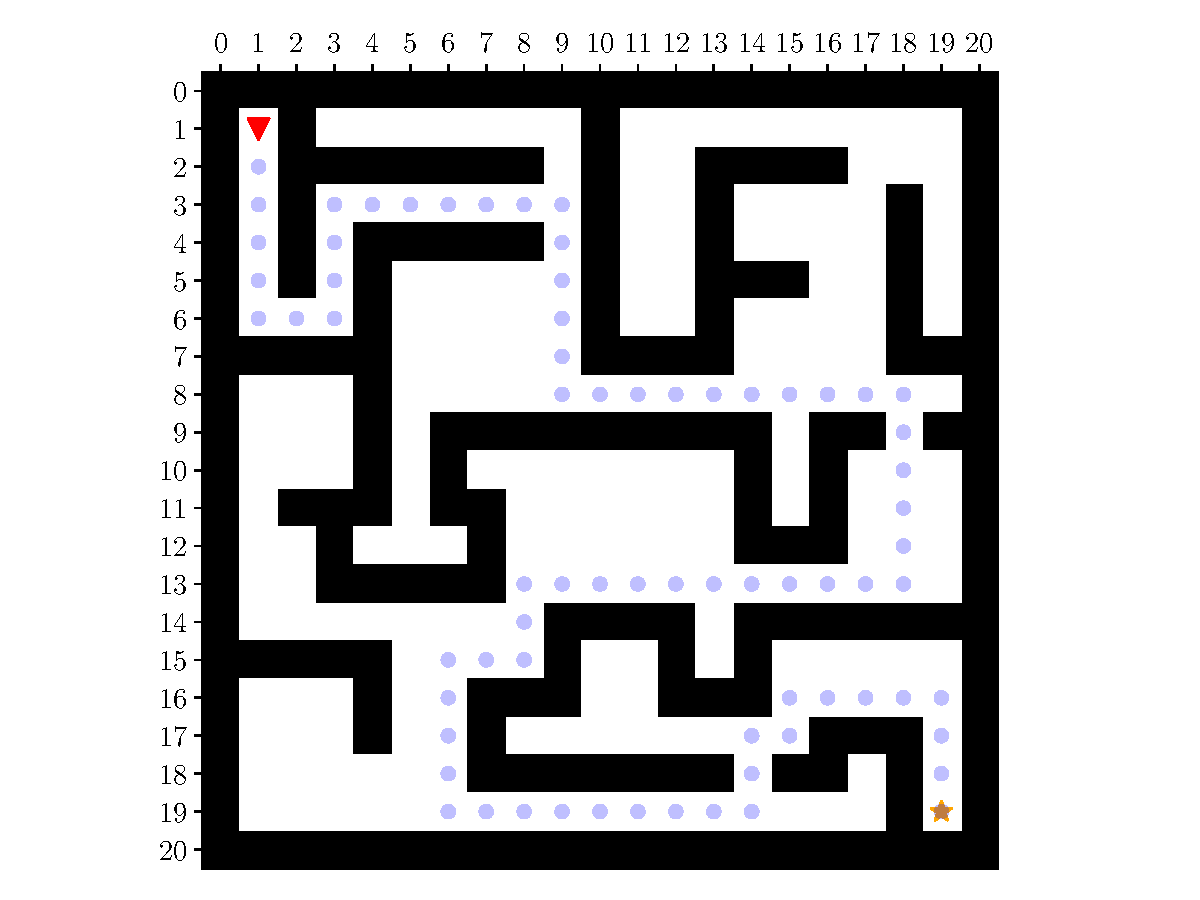
\includegraphics[width=\textwidth]{resources/pdf/05/complex-environment/path.pdf}
        \caption{Complex environment}
        \label{fig:05.path.planning.examples.complex}
    \end{subfigure}
    \caption{Examples of shortest paths (in blue dots) determined, based on the environment representation, via the A* path planning algorithm.}
    \label{fig:05.path.planning.examples}
\end{figure}

In both cases, the algorithm correctly found the shortest path from the starting point to the objective. The execution times\footnote{All execution times mentioned in this work were obtained on the same machine which is described in Appendix \ref{ch:technical.specifications}.} of the algorithm were, in both cases, less than $\SI{1}{\milli\second}$. Since the path is calculated before the drone flies, its execution time is not critical. However, from a perspective where the path could be re-calculated in flight, a fast execution time is nevertheless interesting.

\begin{note}
    In this work, diagonal movements have not been considered. Indeed, the environments considered being corridors, the drone will never really be required to move diagonally.
\end{note}

\subsection{Key points extraction}\label{sec:05.key.points.extraction}

For the purpose of autonomous navigation, it is important that the drone is able to extract information from the path it has to follow. For example, the drone must be able to know whether it should turn left or right at the first crossroads it encounters, whether the staircases are going up or down, etc.

All this information can be extracted based on the environment representation and the path the drone has to follow. This information is called \emph{key points}. In this work, the different key points of an environment considered are turns, crossroads and staircases.

When the drone has determined the shortest path to its objective, it extracts key points. These are tuples consisting of a position and an action, \eg{} the key point \texttt{((1, 1), 'right')} means that there is a key point at position $(1, 1)$ and that it is a turn (or crossroad) where the drone must turn right.

Staircases, and the associated actions, are extracted simply on the basis of knowledge of their position in the environment (given in the \texttt{.txt} file by the symbols \texttt{+} and \texttt{-}, see Table \ref{tab:05.environment.representation.symbols}). Turns and crossroads, on the other hand, are extracted by applying a simple algorithm, on each point that composes the path, that checks the number of free neighbors. If a point has at least two non-aligned free neighbors, it is considered as a key point.

\begin{note}
    One must pay attention that this simple algorithm only works with environment representations where each corridor has a width of one discretized step (for example, the environment shown in Figure \ref{fig:05.indoor.corridor.representation}). For more complex environments, such as those presented in Figure \ref{fig:05.path.planning.examples}, the algorithm must be adapted, else it will consider that each point in an \enquote{open} area is a key point.
\end{note}

The actions associated with each turn are then deduced on the basis of its position, the position of the next point in the path and the orientation of the drone. This can be \texttt{left}, \texttt{right} but also \texttt{forward} if the drone has, for example, to continue straight forward at a crossroad.

By applying this key point extraction procedure to the complex environment of Figure \ref{fig:05.path.planning.examples.complex}, we obtain, as the first key point of the list, \texttt{((6, 1), 'left')}. Indeed, the key point that the drone will meet will be a turn to the left (from its point of view) and located at the position $(6, 1)$.

It is important to note that the key points composing a path are extracted in the order in which the drones will encounter them.

\subsection{Drone position}\label{sec:05.drone.position}

The position and orientation of the drone in the environment representation (red arrow) can be updated based on the actions performed and its current orientation.

When the drone performs the action \texttt{forward}, its position is updated in the environment according to its orientation. For example, in the representation \ref{fig:05.path.planning.examples.simple}, the drone's new position would be $(1, 2)$ and in the representation \ref{fig:05.path.planning.examples.complex}, its new position would be $(2, 1)$.

When the drone performs the action \texttt{left} or \texttt{right} (turn left or right), its orientation is updated according to its current orientation. For example, in Figure \ref{fig:05.path.planning.examples.simple}, the action \texttt{right} would orient the drone towards the South. In Figure \ref{fig:05.path.planning.examples.complex}, this same action would orient the drone towards the West.

It is therefore possible to estimate the position of the drone in the environment solely on the basis of the actions it performs. It should be noted that the update of the position has to be adapted according to the precision of the environment and the movement of the drone. For example, if the precision is $\SI{1}{\meter}$ and the drone moves in steps of $\SI{50}{\centi\meter}$, its position has to be updated in the environment only one action over two.

It is also possible to update the position of the drone in the environment directly on a coordinate basis. This can be used when the drone detects a key point. Knowing the position of the key points of the environment (see Section \ref{sec:05.key.points.extraction}), when the drone detects one, it can be moved to the exact corresponding position in the environment representation.

\subsection{Battery management}\label{sec:05.battery.management}

The battery is a critical issue for drones. Indeed, in small models, such as the Tello EDU, the battery only lasts a few minutes (see Table \ref{tab:04.tello.edu.characteristics}).

In this work, the battery was not considered a major problem because the paths taken by the drone are very short. However, in order to improve the drone's complete autonomy navigation system, it is interesting to take the battery into account when planning paths.

Another work, always carried out within the framework of various works on drones mentioned before, consists in designing charging stations for the drone that work by induction. We could therefore imagine a scenario where these charging stations would be present in the environment. These can be represented via the appropriate symbol (the symbol \texttt{B}, see Table \ref{tab:05.environment.representation.symbols}) when creating an environment representation.

The idea is to check the battery level of the drone before planning a path. Depending on the battery level, the drone can directly reach its objective or go first to a battery station. The adapted path planning algorithm in described in Algorithm \ref{alg:05.path.planning.batteries}.

\begin{algorithm}[H]
    \begin{algorithmic}[1]
        \Function{path}{$start, end$}
            \State Let $d$ be the distance to $end$
            \State Let $max\_d$ be the maximal distance that the drone can travel \label{alg:05.path.planning.batteries.max.d} \\
            \If{$max\_d \geq d$}
                \State \Return \Call{a\_star}{$start, end$}
            \Else
                \State Let $b$ be the farthest reachable battery station \label{alg:05.path.planning.next.station} \\
                \If{$b$ has already been visited} \label{alg:05.path.planning.batteries.already.visited}
                    \State \Return empty path
                \EndIf \\
                \State \Return \Call{a\_star}{$start, b$} + \Call{path}{$b$, $end$}
            \EndIf
        \EndFunction
    \end{algorithmic}
    \caption{Path planning with battery stations.}
    \label{alg:05.path.planning.batteries}
\end{algorithm}

The maximum distance the drone can fly (line \ref{alg:05.path.planning.batteries.max.d} of the Algorithm) can be obtained via its battery level and a simple model. For example, if we know that, with a fully charged battery, the drone can fly $\SI{10}{\minute}$ and that it flies at $\SI{1}{\meter\per\second}$, then it could fly $\SI{600}{\meter}$. This model is, of course, a very simple approximation but can be sufficient, if we take a safety margin, to plan a correct path.

To get the farthest reachable station (line \ref{alg:05.path.planning.next.station} of the Algorithm), the station with the higher distance to the drone but still lower than the maximal distance the drone can travel is chosen.

If the drone has already visited a battery station $b$, the algorithm returns an empty path and stops (line \ref{alg:05.path.planning.batteries.already.visited} of the Algorithm). Indeed, if the drone has to return to a battery station already visited, it means that it can never find a path that can lead it to the objective with sufficient battery level.

This algorithm is greedy: the drone always tries to reach its objective first if its battery allows it, else it tries to go to the farthest battery station in order to recharge as late as possible and arrive at its objective with the maximum amount of battery. It does not always provide the optimal path, especially if there are battery stations that are far from the drone \emph{and} the objective. In the context of the simple tests realized in this work, it is sufficient, but it could be improved, using for example dynamic programming, in a future work.

The Algorithm \ref{alg:05.path.planning.batteries} was applied to the complex environment with, respectively, a battery level of $100\%$, $50\%$ and $20\%$. The results are presented in Figure \ref{fig:05.path.planning.batteries.examples} where the green crosses represent a battery station.

\begin{figure}[H]
    \centering
    \begin{subfigure}[b]{0.32\textwidth}
        \centering
        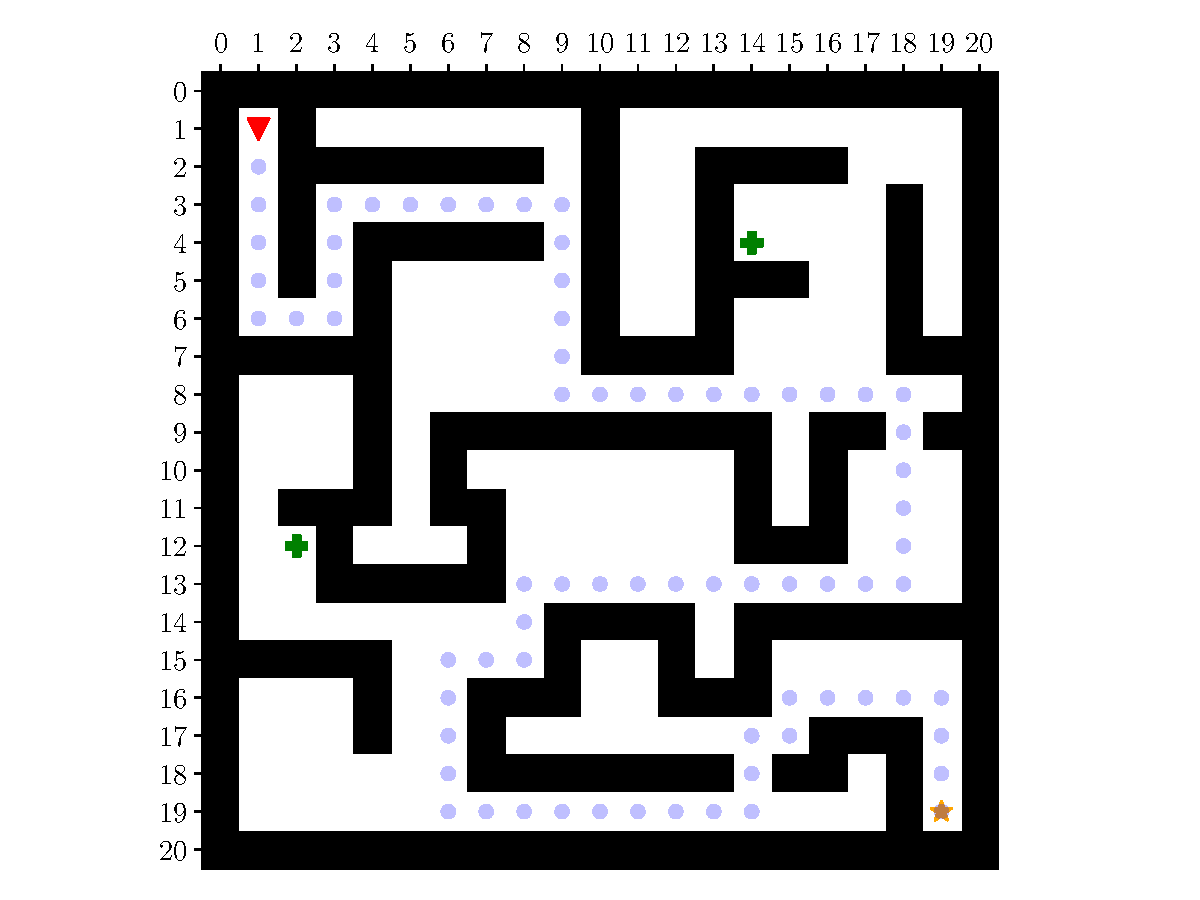
\includegraphics[width=\textwidth]{resources/pdf/05/complex-environment/b100.pdf}
        \caption{Battery level: $100\%$}
    \end{subfigure}
    \hfill
    \begin{subfigure}[b]{0.32\textwidth}
        \centering
        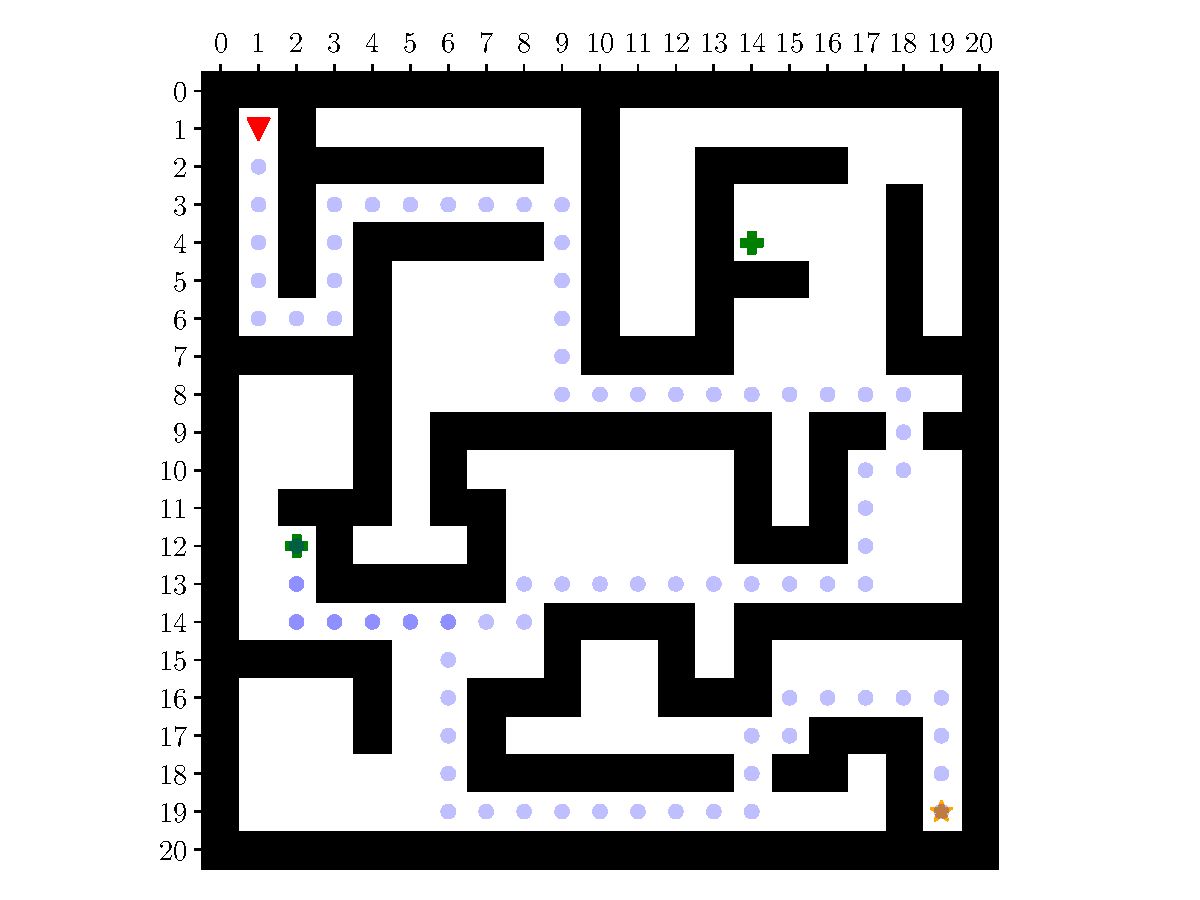
\includegraphics[width=\textwidth]{resources/pdf/05/complex-environment/b50.pdf}
        \caption{Battery level: $50\%$}
    \end{subfigure}
    \hfill
    \begin{subfigure}[b]{0.32\textwidth}
        \centering
        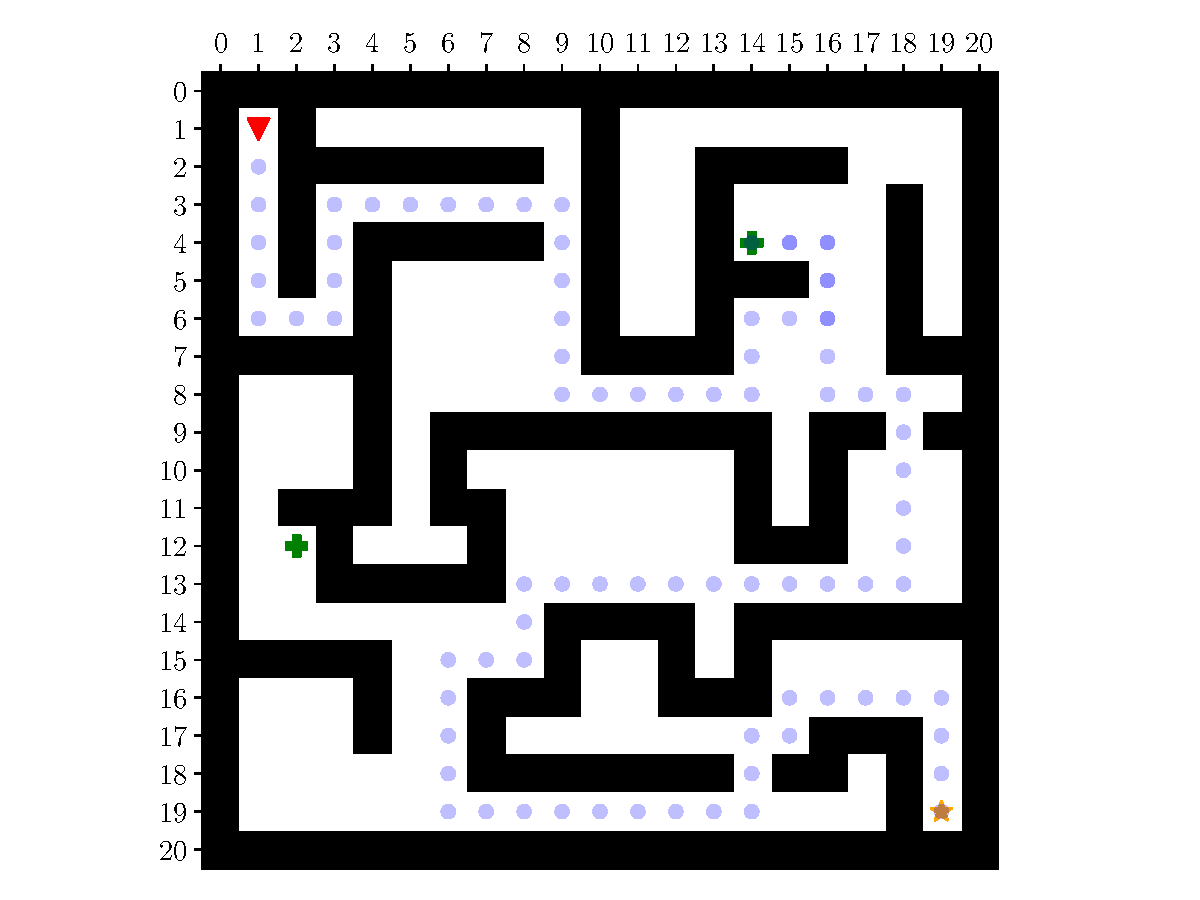
\includegraphics[width=\textwidth]{resources/pdf/05/complex-environment/b20.pdf}
        \caption{Battery level: $20\%$}
    \end{subfigure}
    \caption{Examples of paths determined via the Algorithm \ref{alg:05.path.planning.batteries} for different battery levels.}
    \label{fig:05.path.planning.batteries.examples}
\end{figure}

In the case of a full battery, it can be seen that the drone can go directly to its objective. When the battery is charged to $50\%$, the drone can go to the farthest battery station. This allows it to arrive at its objective at a high battery level. With $20\%$ battery, the drone first passes through the nearest battery station before going to its objective.

\subsection{Staircases and floors management}\label{sec:05.staircases.floors.management}

The last feature is the management of staircases and floors. Indeed, an environment can contains several floors linked with staircases.

Staircases are considered as key points of the environment and can be represented using the appropriate symbols (\texttt{+} and \texttt{-}, see Table \ref{tab:05.environment.representation.symbols}).

The representation of an environment being in two dimensions, it is not possible to manage several floors in a single representation. The solution adopted in this work is to represent each floor via a different representation. When a staircase is reached by the drone, the corresponding representation of the next floor is loaded into memory and replaces the current representation used. A new path is determined and the drone can continue its navigation.

\section{Application to this work}

Environment representations have been made for each of the environments considered in this work.

\subsection{Indoor Corridor}

Based on the aerial view of the environment presented in Figure \ref{fig:03.aerial.views}, a representation of the Indoor Corridor environment has been realized in Figure \ref{fig:05.indoor.corridor.representation}.

\begin{figure}[H]
    \centering
    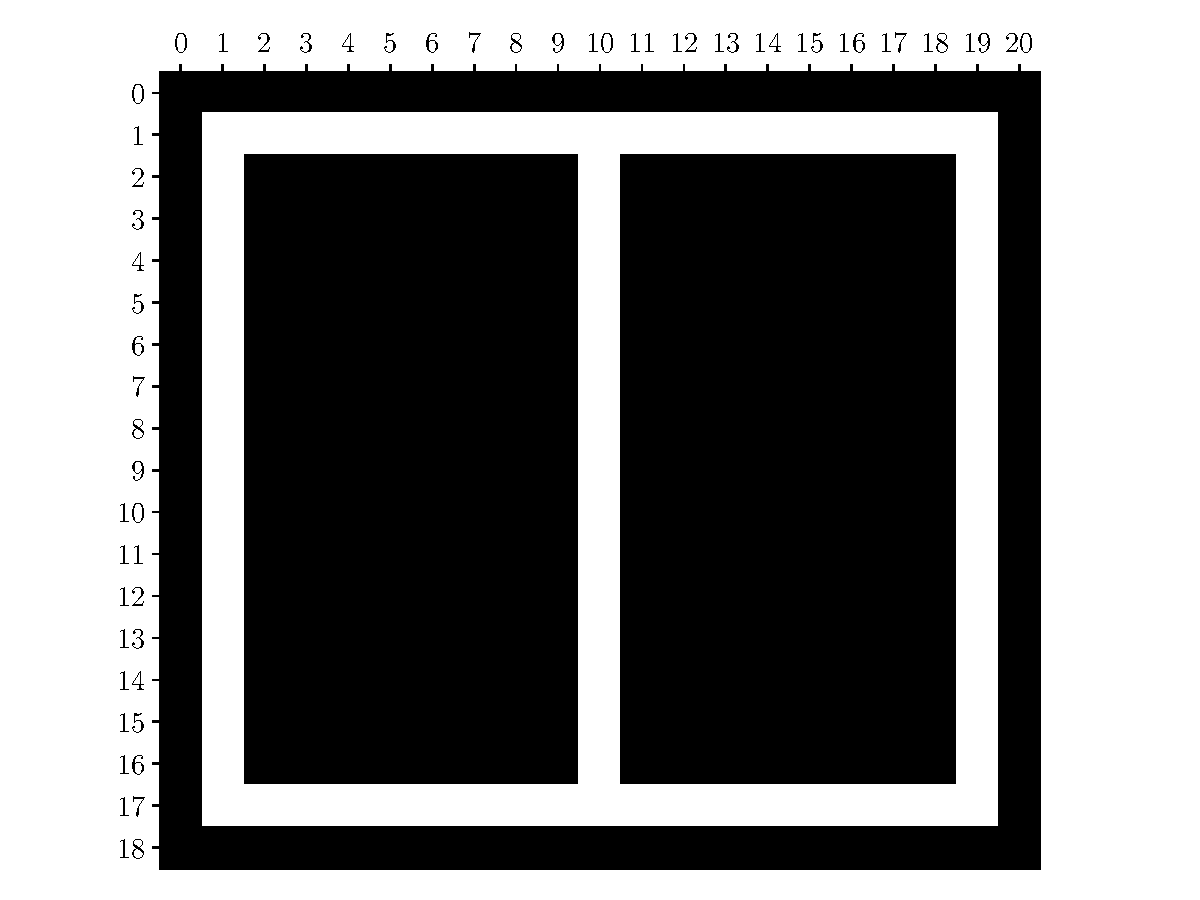
\includegraphics[width=0.5\textwidth]{resources/pdf/05/indoor-corridor/0.pdf}
    \caption{Visual representation of the Indoor Corridor simulated environment.}
    \label{fig:05.indoor.corridor.representation}
\end{figure}

A small video illustrating a simple usage of this environment representation is available via the following link: \url{https://youtu.be/fyyEQhqTZp8}.

\subsection{Indoor Staircase}

Also on the basis of the aerial view of the environment presented in Figure \ref{fig:03.aerial.views}, a simple representation was made. As the Indoor Staircase environment has a staircase, and therefore a floor, two representations were made: floor 0 and floor 1 (Figure \ref{fig:05.indoor.staircase.representation}).

\begin{figure}[H]
    \centering
    \begin{subfigure}[b]{0.58\textwidth}
        \centering
        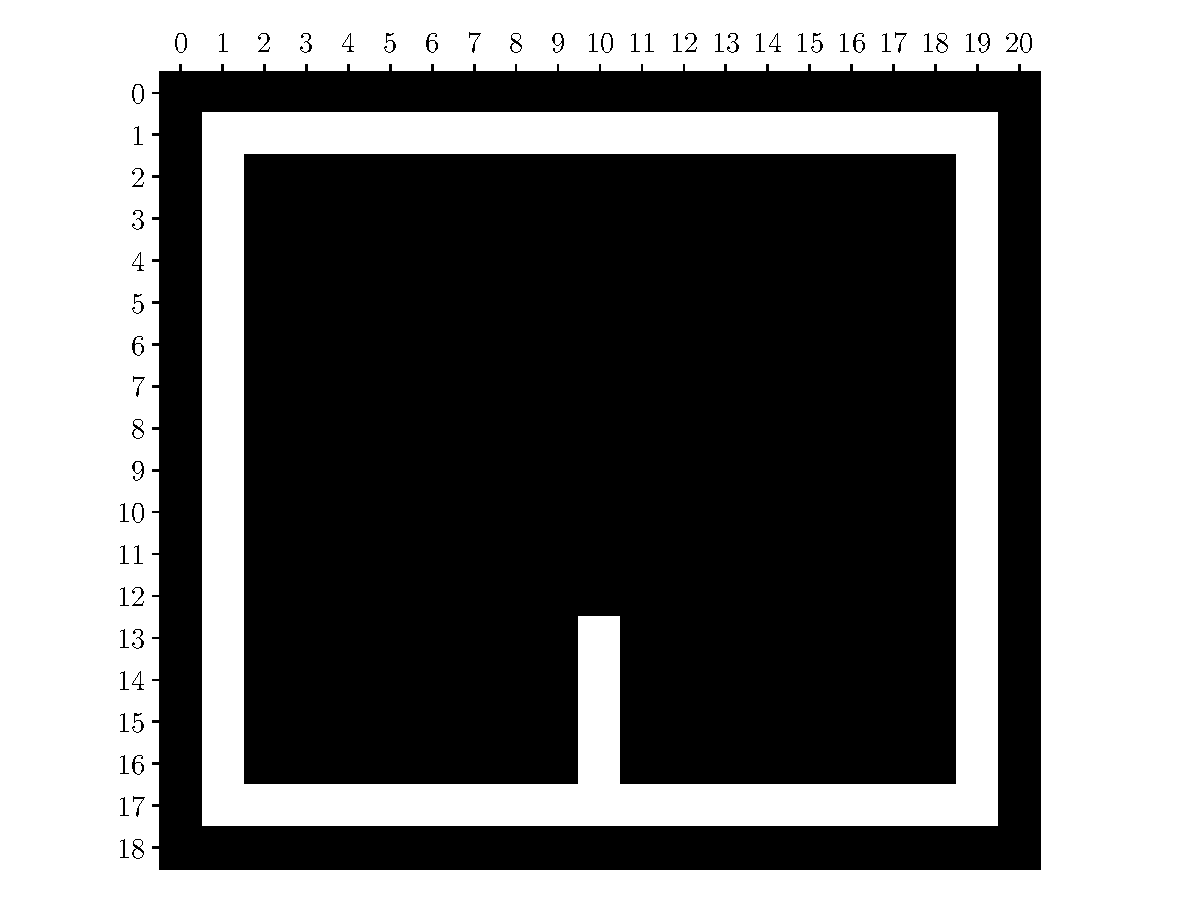
\includegraphics[width=0.8\textwidth]{resources/pdf/05/indoor-staircase/0.pdf}
        \caption{Floor 0}
    \end{subfigure}
    \hfill
    \begin{subfigure}[b]{0.38\textwidth}
        \centering
        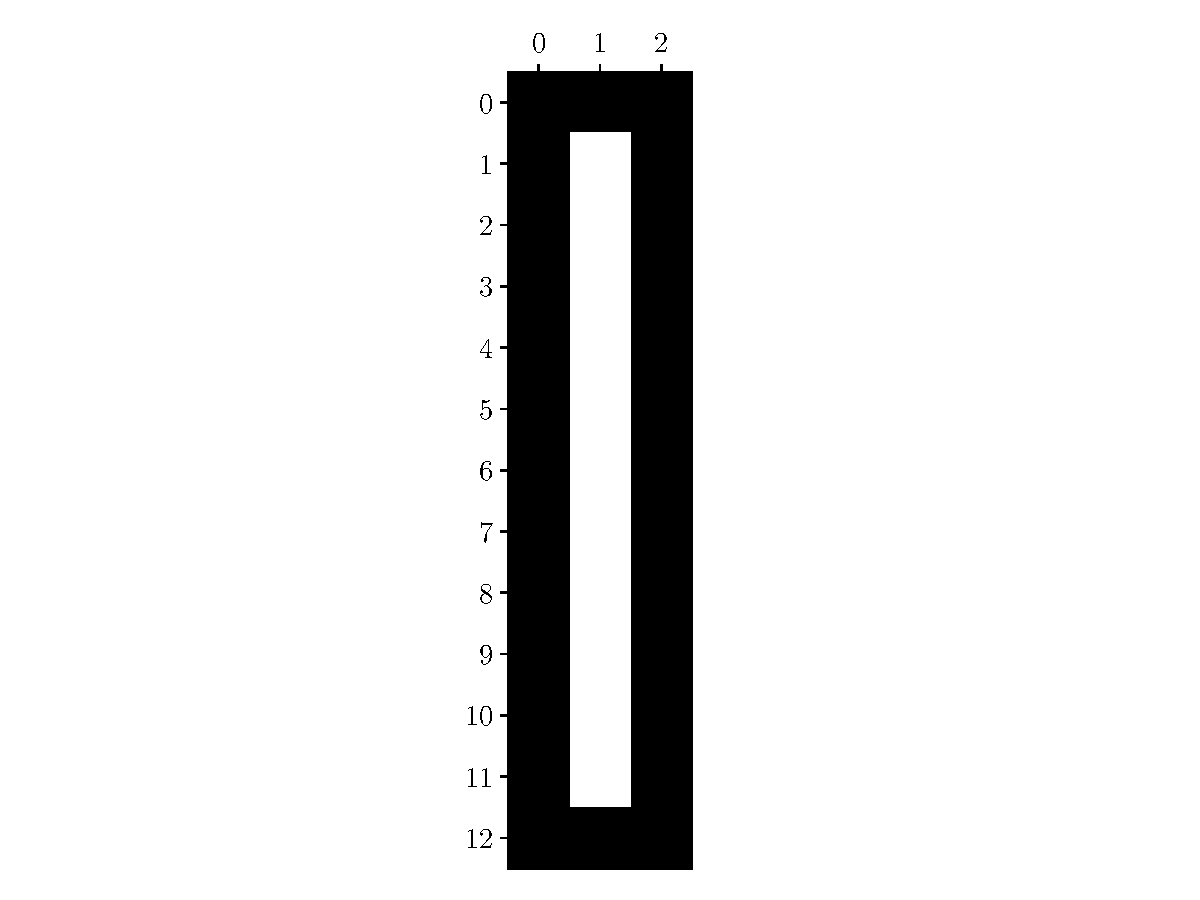
\includegraphics[width=0.313\textwidth]{resources/pdf/05/indoor-staircase/1.pdf}
        \caption{Floor 1}
    \end{subfigure}
    \caption{Visual representation of the Indoor Staircase simulated environment.}
    \label{fig:05.indoor.staircase.representation}
\end{figure}

\subsection{Montefiore Institute}\label{sec:05.montefiore.institute}

On the basis of small plans available at the entrance of the building, a representation of the Montefiore Institute (floor -1) has been made (Figure \ref{fig:05.b28.representation}).

\begin{figure}[H]
    \centering
    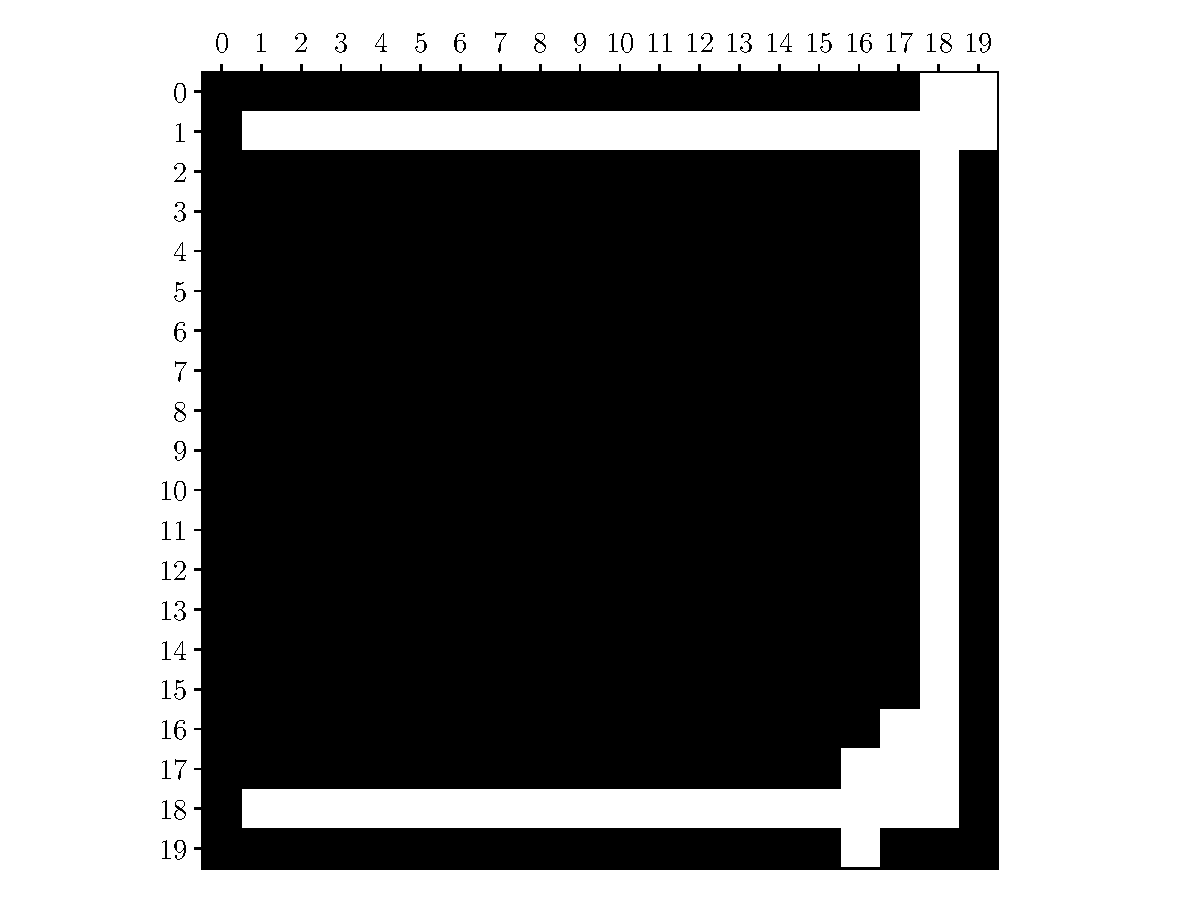
\includegraphics[width=0.5\textwidth]{resources/pdf/05/b28/basement.pdf}
    \caption{Visual representation of floor -1 of the Montefiore Institute of the University of Liège.}
    \label{fig:05.b28.representation}
\end{figure}
